Certainly! Below is an example of how you can generate a TikZ LaTeX diagram to illustrate both parts of your prompt: an instance of MCR (Multi-Objective Coverage Reaching) with 4 obstacles, and the corresponding graph transformation.

```latex
\documentclass{standalone}
\usepackage{tikz}

\begin{document}

% Part (a): Instance of MCR with 4 obstacles
\begin{figure}[h]
    \centering
    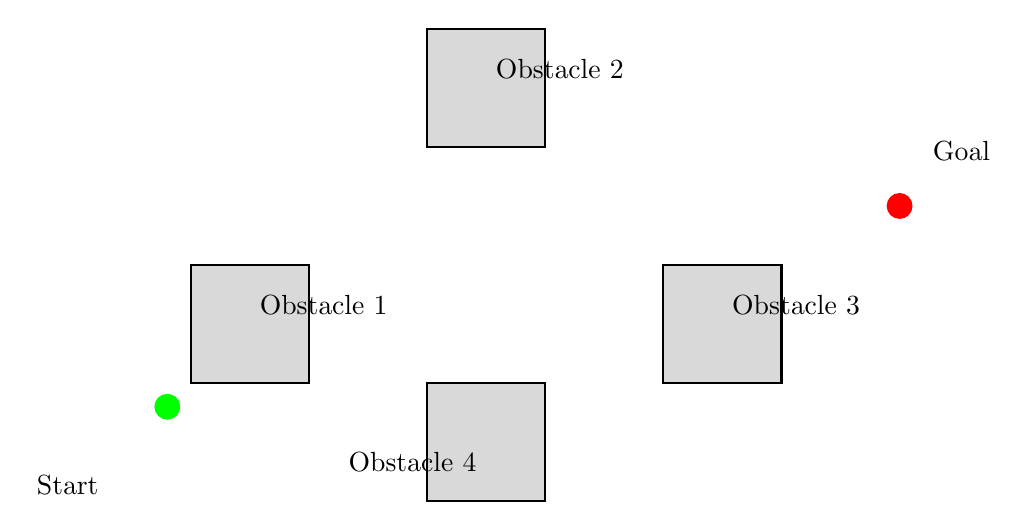
\begin{tikzpicture}[scale=1.5]
        % Drawing the obstacles
        \draw[thick, fill=gray!30] (0,0) rectangle (1,1); % Obstacle 1
        \draw[thick, fill=gray!30] (2,2) rectangle (3,3); % Obstacle 2
        \draw[thick, fill=gray!30] (4,0) rectangle (5,1); % Obstacle 3
        \draw[thick, fill=gray!30] (2,-1) rectangle (3,0); % Obstacle 4

        % Drawing start and goal locations
        \filldraw[green, thick] (-0.2, -0.2) circle (0.1); % Start location
        \filldraw[red, thick] (6, 1.5) circle (0.1); % Goal location

        % Adding labels
        \node at (0.5, 0.5) [above right] {Obstacle 1};
        \node at (2.5, 2.5) [above right] {Obstacle 2};
        \node at (4.5, 0.5) [above right] {Obstacle 3};
        \node at (2.5, -0.5) [below left] {Obstacle 4};

        \node at (-0.7, -0.7) [below left] {Start};
        \node at (6.2, 1.8) [above right] {Goal};
    \end{tikzpicture}
    \caption{(a) An instance of MCR with 4 obstacles. Start and goal locations are shown in green and red, respectively.}
\end{figure}

% Part (b): Graph transformation of the MCR problem
\begin{figure}[h